\documentclass[11pt,a4paper]{article}

\usepackage[T1]{fontenc}
\usepackage[utf8]{inputenc}
\usepackage[frenchb]{babel}

\usepackage{fancyhdr} % headers
\usepackage[usenames,dvipsnames]{color} % colors
\usepackage{graphicx} % images
\usepackage{listings} % source code
\usepackage{titling} % meta-infos
\usepackage{courier} % courier font
\usepackage{fullpage} % full page layout
\usepackage{titlesec} % title customization
\usepackage{parskip} % paragraphs spacing
\usepackage{amsmath}
\usepackage{enumitem}
\usepackage{listings} % Affichage de code source
\usepackage[bottom]{footmisc} % Alignement BOTTOM des footnotes
%\usepackage{showframe} % layout debug

\usepackage{float}
\restylefloat{figure}

\topmargin -10mm
\headsep 5mm
\headheight 10mm

\linespread{1.1}
\renewcommand{\arraystretch}{1.3}

\setlength\parindent{0pt}
\setlength{\unitlength}{1cm}
\setlength{\droptitle}{-1.6cm}

\pagestyle{fancy}
\fancyhf{}
\cfoot{\thepage}

\def \doccourse { ASD2 }
\def \doctitle { Labo 04 - Table de Hashage }
\author{Kevin Do Vale \and Aleksandar Milenkovic \and David Cruchon}

\rhead{ \theauthor \\ \today}
\lhead{\doccourse \\ \doctitle }
\title{{\normalsize \doccourse} \\ \doctitle }

\begin{document}

\lstset{language=C++}
\maketitle
\vspace{1em}

\section{Introduction}
Ce laboratoire est composé de deux parties.
Dans la première partie, nous avons pour but de comparer les 6 différentes fonctions de hashage fournie dans la donnée. Nous devons également évaluer les performances de chaque fonctions de hashage sur différents jeux de donnée.

\section{Analyse partie 1}
Cette première partie compare les différentes fonctions de hashage fournie dans la donnée. A savoir :
\textbf{atoi} pour la classe \textit{DirectoryInt}, \textbf{atol} pour la classe \textit{DirectoryLong}, 3 fonctions de \textbf{compression polynomiales} pour la classe \textit{DirectoryPol<X>,} \textbf{hash} pour la classe \textit{DirectoryStl}, \textbf{sha256} pour la classe \textit{DirectorySha256} et une fonction custom \textbf{CityHash64} pour la classe \textit{DirectoryCity}.

Les tests ont été effectués avec les deux listes fournies. La première comporte 10'000 éléments et la seconde 1'000'000 d'éléments. De plus, nous avons également pris en considération le facteur MAX\textunderscore LOAD\textunderscore FACTOR\footnote{Pour répondre à la question, ce facteur est définit à 1.0 dans la STL. Les collisions sont gérées par "collision chain".}.

Les deux graphiques ci-dessous représentent les temps moyen d'insertion et de recherche. Attention, les temps sont superposés. Ce qui nous intéresse ici, c'est de pouvoir déceler des "anomalies" sur les temps d'exécution.

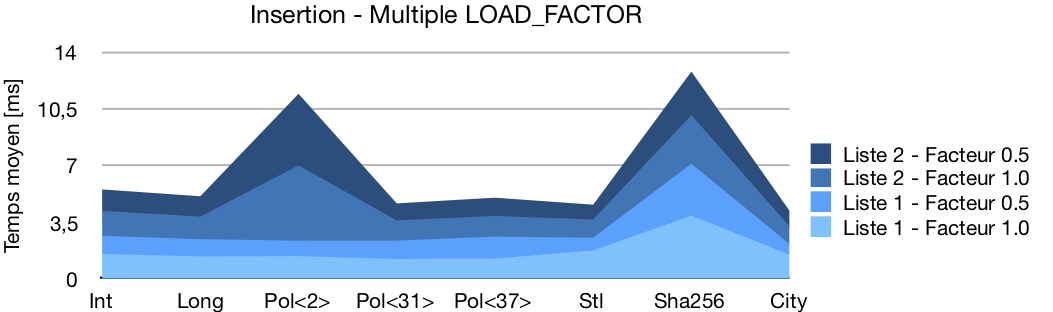
\includegraphics[width=\textwidth,keepaspectratio]{insert_chart.png}
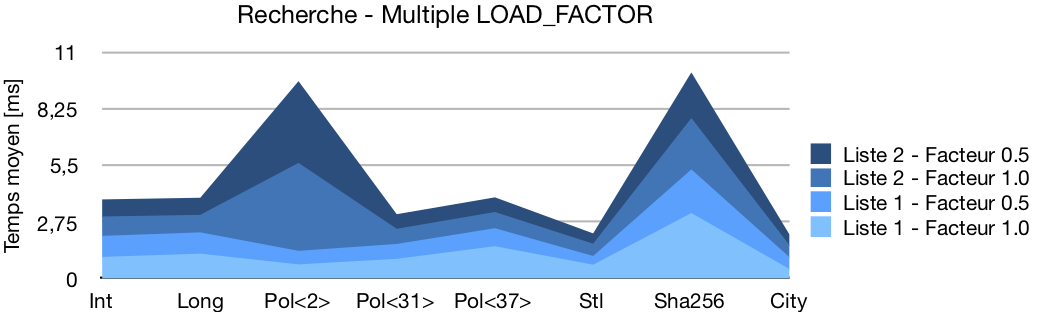
\includegraphics[width=\textwidth,keepaspectratio]{search_chart.png}

Ces deux premiers graphiques nous permettent de mettre en évidence plusieurs choses. La première, c'est un temps moyen d'exécution anormalement plus élevé sur la deuxième liste (1'000'000 d'éléments) lors de l'utilisation de fonction de hashage polynomiale avec 2 comme nombre premier. Deuxièmement, on voit clairement que la fonction de hashage utilisant sha256 est plus gourmande en terme de temps d'exécution.

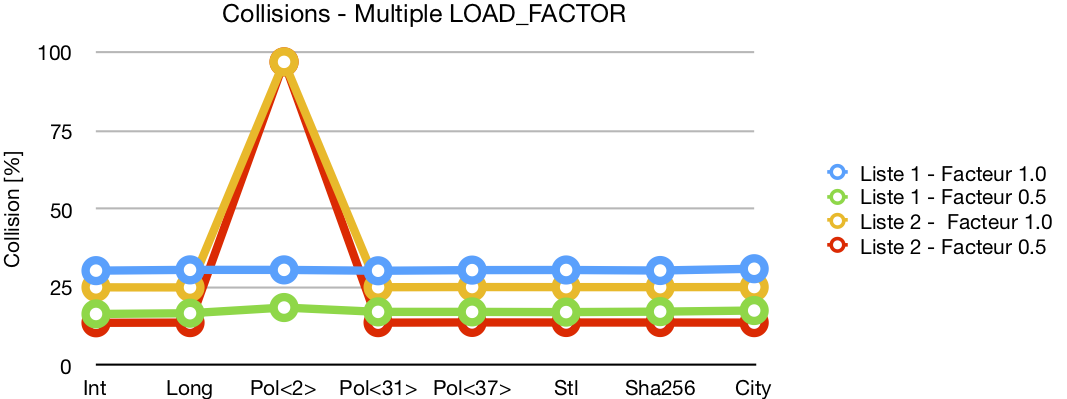
\includegraphics[width=\textwidth,keepaspectratio]{collisions_chart.png}

Dans ce graphique, on observe clairement que sur un nombre d'élément élevé (ici 1'000'000) la fonction de hashage utilisant une compression polynomiale avec comme paramètre 2 comme nombre premier, le taux de collision approche les 100\%.

\section{Analyse partie 2}
L'implémentation fournie n'est pas optimale car la clé utilisée (le nom de la personne) ne permet pas d'identifier de manière distincte une personne. Ceci va entraîner un haut taux de collision. En effet, dans les tests effectués, nous trouvons un taux de collision d'environ \textbf{64\%}.

Une  première solution serait de rendre unique la clé utilisée. Par exemple, une composition du \textbf{nom}, \textbf{prénom} et \textbf{date de naissance}. Dans ce cas, la propriété genre n'apporterait pas grand chose sur la composition de la clé. En effet, cette propriété peux prendre seulement deux valeurs composé d'un seul caractère : F ou H. En testant cette première implémentation, nous tombons à un taux de collision de \textbf{30\%}.

\begin{lstlisting}[frame=single] 
std::string key = d.getBirthday() + d.getName() + d.getFirstname();
return std::hash<std::string>()(key);
\end{lstlisting}

Une deuxième solution serait d'implémenter une fonction de hash utilisant une compression polynomiale sur la même clé utilisée dans la première solution. A savoir \textbf{nom + prénom + date de naissance}. Nous utilisons \textbf{33} comme nombre premier. Les tests ne démontre pas de grande différence avec la première solution. Nous restons à un taux de collision d'environ \textbf{30\%}.

\begin{lstlisting}[frame=single] 
size_t h = 0L;
size_t z = 33; // Choix du nombre premier. Page 16 du polycop.

for (int i = 0; i < key.length(); ++i) {
	h = (z * h) + key[i];
}

return h;
\end{lstlisting}

Dans les deux solutions, les tests sont effectués avec MAX\textunderscore LOAD\textunderscore FACTOR à 1. Lorsque nous diminuons ce facteur, les taux de collision tombe de manière significative. En effet, pour les deux solutions, lorsque nous définissons ce facteur à 0.5, le taux de collision n'est plus que de 16\%. A contrario du nombre de \textit{bucket}\footnote{Slot ou alvéole en français. Il s'agit du contenant "choisi" par le résultat du Hash pour stocker la valeur } qui augmente considérablement. Il est donc important de trouver un juste milieu.
\section{Conclusion}
Ce laboratoire se rapproche plus d'une compréhension des résultats fournis par la données qu'un laboratoire technique. Mise à part la seconde partie, où l'on devais fournir une implémentation pour la classe DirectoryWithoutAVS. Deux solutions ont été proposées mais nous sommes certains qu'il y ai encore mieux à faire afin de réduire le taux de collision et de réduire le nombre de buckets vide.

\end{document}
